% Standard Article Definition
\documentclass[]{article}

% Page Formatting
\usepackage[margin=1in]{geometry}
\setlength\parindent{0pt}

% Graphics
\usepackage{graphicx}

% Math Packages
\usepackage{physics}
\usepackage{amsmath, amsfonts, amssymb, amsthm}
\usepackage{mathtools}

% Extra Packages
\usepackage{pdfpages}
\usepackage{hyperref}
% \usepackage{listings}

% Section Heading Settings
\usepackage{enumitem}
% \renewcommand{\theenumi}{\alph{enumi}}
\renewcommand*{\thesection}{Problem \arabic{section}}
\renewcommand*{\thesubsection}{\alph{subsection})}
\renewcommand*{\thesubsubsection}{}%\quad \quad \roman{subsubsection})}

\newcommand{\Problem}{\subsubsection*{\textbf{PROBLEM:}}}
\newcommand{\Solution}{\subsubsection*{\textbf{SOLUTION:}}}
\newcommand{\Preliminaries}{\subsubsection*{\textbf{PRELIMINARIES:}}}

%Custom Commands
\newcommand{\N}{\mathbb{N}}
\newcommand{\Z}{\mathbb{Z}}
\newcommand{\Q}{\mathbb{Q}}
\newcommand{\R}{\mathbb{R}}
\newcommand{\C}{\mathbb{C}}

\newcommand{\SigAlg}{\mathcal{S}}

\newcommand{\Rel}{\mathcal{R}}

% \newcommand{\toI}{\xrightarrow{\textsf{\tiny I}}}
% \newcommand{\toS}{\xrightarrow{\textsf{\tiny S}}}
% \newcommand{\toB}{\xrightarrow{\textsf{\tiny B}}}

\newcommand{\divisible}{ \ \vdots \ }
\newcommand{\st}{\ : \ }

% Theorem Definition
\newtheorem{definition}{Definition}
\newtheorem{assumption}{Assumption}
\newtheorem{theorem}{Theorem}
\newtheorem{lemma}{Lemma}
\newtheorem{proposition}{Proposition}
\newtheorem{remark}{Remark}
% \newtheorem{example}{Example}
% \newtheorem{counterExample}{Counter Example}


%opening
\title{MATH 6301 Real Analysis I \\ Homework 4}
\author{Jonas Wagner\\ jonas.wagner@utdallas.edu}
\date{2022, October 27\textsuperscript{th}}

\begin{document}

\maketitle

\tableofcontents

\includepdf[pages={2}]{math6301a4-2022.pdf}

% Problem 1 ----------------------------------------------
\newpage
\section{}
\Problem
Assume that $U \subset \R^n$ is an open set and $f \st U \to \R$ is a differentiable function.
Show that for every $k = 1,2,\dots,n$, the partial derivative \[
    \pdv{f}{x_k} \st U \to \R
\] is $\mathcal{B}_n$-measurable (here $\mathcal{B}_n$ stands for the $\sigma$-algebra of Borel sets in $\R^n$).

\Preliminaries
\begin{definition}
    Let $\SigAlg \subset P(X)$ is a $\sigma$-algebra and $E \in \SigAlg$.
    The function $f : E \to \overline{\R}$ is called \emph{\underline{measurable}} relative to $\SigAlg$ (i.e. $\SigAlg$-measurable) iff \[
        \forall_{a \in \R} f^{-1}(a,\infty] := \{x \in E \st f(x) > a\} \in \SigAlg
    \] 
\end{definition}
\begin{remark}
    Assume that $f : E \to \overline{\R}$, $E \in \SigAlg \subset P(X)$ is $\SigAlg$-measurable.
    Then the following are also $\SigAlg$-measurable
    \begin{enumerate}
        \item $f^2 : E \to \overline{R}$
        \item $\abs{f} : E \to \overline{R}$
        \item $\frac{1}{f} : E \to \overline{R}$
        \item $a \cdot f : E \to \overline{R}, \ a \in \R$
    \end{enumerate}
\end{remark}
\begin{definition}
    Let $U \subset \R^n$ and $f \st U \to \R$ be a differentiable function.
    The \emph{\underline{partial derivative}} $\pdv{f}{x_k}$ is defined as follows \[
        \pdv{f}{x_k} := \lim_{n\to\infty} \cfrac{
            f \qty(
                % \mqty[x_1 \\ \vdots \\ x_k + 1/n \\ \vdots \\ x_n]
                x_1, 
                \cdots, x_k + 1/n, \cdots
                , x_n
            ) - f \qty(
                % \mqty[x_1 \\ \vdots \\ x_k \\ \vdots \\ x_n]
                x_1, 
                \cdots, x_k, \cdots
                , x_n
            )}{1/n}
    \]
\end{definition}

\Solution
Let $U \subset \R^n$ and $f \st U \to \R$ be a differentiable function.
The partial derivative, $\pdv{f}{x_k}$, can be increasingly estimated by the sequence of simple functions where for each borel-set region $(a,b) \in \mathcal{B}_n$ the simple function value of $[\eval{\pdv{f}{x_k}}_{(a,b)}]_i$ is defined by \[
    \cfrac{
        f\qty(
            a_1, \cdots, a_k + 1/i, \cdots, a_n
        ) - f \qty(
            a_1, \cdots, a_k, \cdots, a_n
        )
        }{
            1/i
        }
\] Since this simple function can approximate $\pdv{f}{x_k} \forall_{k = 1,\dots,n}$, it is $\mathcal{B}_n$-measurable.

% Problem 2 ----------------------------------------------
\newpage
\section{}
\Problem
Let $X$ be a space and $\SigAlg \subset \mathcal{P}(X)$ a $\sigma$-algebra in $X$. 
We say that the map $f : X \to \R^n$ is $\SigAlg$-measurable if and only if \[
    \forall_{V \in \mathcal{B}_n} f^{-1}(V) \in \SigAlg
\] Assume that $f : X \to \R^n$ is a map that for all $v \in \R^n$ the function $\phi_y(x):= f(x) \bullet v$, $x \in X$, is $\SigAlg$-measurable.
Show that the map $f$ is $\SigAlg$-measurable.

% \Preliminaries

\Solution
In order for $\phi_y(x)$ to be measurable each dimension of the dot product must be measurable. (i.e)\[
    \phi_y(x) = f_1(x) \cdot v_1 + \cdots + f_n(x) \cdot v_n \ \text{measurable} \ \implies f_i(x) \ \text{measurable} \ \forall_{i = 1\to n}
\] we now know that each dimension measurable in $\mathcal{B}$, therefore $f$ is measurable in $\mathcal{B}_n$.

% Problem 3 ----------------------------------------------
\newpage
\section{}
\Problem
Let $X$ be a bounded set in Banach space $\mathcal{E}$. 
We define the following function $\mu^* : \mathcal{P}(X) \to \R$ by \[
    \mu^* (A) := \inf\qty{
        r > 0 \st \exists_{x_1,x_2,\dots,x_k \in X} A \subset \bigcup_{j=1}^{k} B_r(x_j)
    }, A \subset X
\] where $B_r(x_0):= \{x \in \mathcal{E} \st \norm{x - x_0} < r\}$. 
Verify if the function $\mu^*$ is an outer measure on $X$ and if it is check if it is a metric outer measure.

(The function $\mu^*$ defined above is called a \emph{measure of non-compactness}. 
Can you guess what would be $\mu^*$ if $\mathcal{E} = \R^n$?)

\Preliminaries
\begin{definition}
    An \textbf{outer measure} $\mu \st \mathcal{P}(X) \to [0,\infty]$ must satisfy the following:
    \begin{itemize}
        \item Null empty set: $\mu(\emptyset) = 0$
        \item Monotone: $A,B\subset X \st A \subseteq B \implies \mu(A) \leq \mu(B)$
        \item For arbritrary subsets $B_1,B_2,\dots,\subset X$,\[
            \mu \qty(\bigcup_{j=1}^{\infty} B_j) \leq \sum_{j=1}^{\infty} \mu(B_j)
        \]
    \end{itemize}
\end{definition}

\Solution
We show that $\mu^*$ is an outer measure as follows:
\begin{itemize}
    \item Null empty set: \[
        \mu*(\emptyset) = \inf\qty{
            r > 0 \st \exists_{x_1,x_2,\dots,x_k \in X} \emptyset \subset \bigcup_{j=1}^{k} B_r(x_j)
        } =        
        \inf{\emptyset} = 0
    \]
    \item Monotone: %$A,B\subset X \st A \subseteq B \implies \mu(A) \leq \mu(B)$
    \begin{align*}
        A_1,A_2 \subset X, A_1 \subseteq A_2 &\implies \mu(A_1) \leq \mu(A_2)\\
        &\implies \inf\qty{
            r > 0 \st \exists_{x_1,x_2,\dots,x_k \in X} A_1 \subset \bigcup_{j=1}^{k} B_r(x_j)
        } 
        \\ &\qquad \qquad \leq \inf\qty{
            r > 0 \st \exists_{x_1,x_2,\dots,x_k \in X} A_2 \subset \bigcup_{j=1}^{k} B_r(x_j)
        }
    \end{align*}
    Since $A_1 \subseteq A_2$, the set of $r$ for the first $\inf$ will allways be containted in the secound one.
    (i.e.)\[
        \qty{
            r > 0 \st \exists_{x_1,x_2,\dots,x_k \in X} A_1 \subset \bigcup_{j=1}^{k} B_r(x_j)
        } \subseteq \qty{
            r > 0 \st \exists_{x_1,x_2,\dots,x_k \in X} A_2 \subset \bigcup_{j=1}^{k} B_r(x_j)
        }
    \] therefore $\mu(A_1) \leq \mu(A_2)$
    
    \item %For arbritrary subsets $B_1,B_2,\dots,\subset X$,\[
    %     \mu \qty(\bigcup_{j=1}^{\infty} B_j) \leq \sum_{j=1}^{\infty} \mu(B_j)
    % \]
    Let $A_1,A_2,\dots,\subset X$ be arbritrary, \[
        \mu \qty(\bigcup_{j=1}^{\infty} A_j) \leq \sum_{j=1}^{\infty} \mu(A_j)
    \]\[
        \mu \qty(\bigcup_{j=1}^{\infty} A_j) =
        \inf\qty{
            r > 0 \st \exists_{x_1,x_2,\dots,x_k \in X} \bigcup_{j=1}^{\infty} A_j \subset \bigcup_{j=1}^{k} B_r(x_j)
        }
    \]\[
        \sum_{j=1}^{\infty} \mu(A_j) = 
        \sum_{j=1}^{\infty} \inf\qty{
            r > 0 \st \exists_{x_1,x_2,\dots,x_k \in X} A_j \subset \bigcup_{j=1}^{k} B_r(x_j)
        }
    \] Clearly, $\mu \qty(\bigcup_{j=1}^{\infty} A_j) \leq \sum_{j=1}^{\infty} \mu(A_j)$ since the common ball radius that contains the union of all subsets will be less then the sum of each individual subsets ball radius. 
    It ends up like $\max{r_1,r_2,\dots,r_k} \leq \sum_{i=1}^{k} r_k$.

    This isn't much of a metric outer measure though

    Within $\R^n$, $\mu^*$ doesn't mean much though as every bounded closed set is compact so it just becomes $0$ or $\infty$ as a test of boundedness or not.
\end{itemize}



% Problem 4 ----------------------------------------------
\newpage
\section{}
\Problem
For two given spaces $X$ and $Y$ and assume that $\mu_1^* \st \mathcal{P}(X) \to \overline{\R}$ and $\mu_2^* \st \mathcal{P}(Y) \to \overline{\R}$ are two outer measures.
Define the function $\nu^* \st \mathcal{P}(X \cross Y) \to \overline{\R}$ by \[
    \nu^*(C) := \inf \qty{
        \sum_{k=1}^{\infty} \mu_1^*(A_k) \mu_2^*(B_k) \st C \subset \bigcup_{k=1}^{\infty} A_k \cross B_k, 
        \ A_k \subset X, 
        \ B_k \subset Y
    }
\]
Check if the function $\nu^*$ is an outer measure on $X \cross Y$.

% \Preliminaries


\Solution
We test $\nu^*$ as an outer measure on $X \cross Y$ as follows:
\begin{itemize}
    \item Null empty set: %$\mu(\emptyset) = 0$
    \[
        \nu^*(\emptyset) = \inf \qty{
            \sum_{k=1}^{\infty} \mu_1^*(\emptyset) \mu_1^*(\emptyset)
        } = 0
    \]
    \item Monotone: %$A,B\subset X \st A \subseteq B \implies \mu(A) \leq \mu(B)$
    \begin{align*}
        C_1 \subseteq C_2 &\implies \inf \qty{
            \sum_{k=1}^{\infty} \mu_1^*(A_k) \mu_2^*(B_k) \st C_1 \subset \bigcup_{k=1}^{\infty} A_k \cross B_k, 
            \ A_k \subset X, 
            \ B_k \subset Y
        } \\
        &\qquad \qquad \leq \inf \qty{
            \sum_{k=1}^{\infty} \mu_1^*(A_k) \mu_2^*(B_k) \st C_2 \subset \bigcup_{k=1}^{\infty} A_k \cross B_k, 
            \ A_k \subset X, 
            \ B_k \subset Y
        }
    \end{align*} Since $C_1 \subseteq C_2$, every $C_1 \subseteq C_2 \subset \bigcup_{k=1}^{\infty} A_k \cross B_k$ so therefore $\mu(A_1) \leq \mu(A_2)$

    \item %For arbritrary subsets $B_1,B_2,\dots,\subset X$,\[
    %     \mu \qty(\bigcup_{j=1}^{\infty} B_j) \leq \sum_{j=1}^{\infty} \mu(B_j)
    % \]
    Let $C_1,C_2,\dots,\subset X$ be arbritrary, \[
        \nu^* \qty(\bigcup_{j=1}^{\infty} C_j) \leq \sum_{j=1}^{\infty} \nu^*(C_j)
    \] We've established that $C_1 \subseteq C_2 \subset \bigcup_{k=1}^{\infty} A_k \cross B_k$, and we use this same logic to show that $\bigcup_{j=1}^{\infty} C_j \subset \bigcup_{j=1}^{\infty} \qty(\bigcup_{k=1}^{\infty} A_k \cross B_k)_j$ and therefore the $\sum_{k=1}^{\infty} \mu_1(A_k) \mu_2(B_k)$ of the union is less then $\sum_{j=1}^{k}\qty(\sum_{k=1}^{\infty} \mu_1^*(A_k) \mu_2^*(B_k))$.
\end{itemize}


% Problem 5 ----------------------------------------------
\newpage
\section{}
\Problem
A set $I \subset \R^n$ is called an \emph{interval} in $\R^n$ if there exists $a_1 \leq b_1, a_2 \leq b_2, \dots, a_n \leq b_n$ such that \[
    (a_1,b_1) \cross (a_2,b_2) \cross \cdots, \cross (a_n,b_n) \subset I \subset [a_1,b_2] \cross [a_2,b_2] \cross \cdots \cross [a_n,b_n]
\]
We denote by $\mathcal{F}$ the family of all intervals in $\R^n$.
Consider the set \[
    X := [c_1,d_1] \cross [c_2,d_2] \cross \cdots \cross [c_n,d_n], \quad c_k < d_k
\]
Is the family $\mathcal{R} \subset \mathcal{P}(X)$, given by \[
    \mathcal{R} := \qty{
        A \subset X : 
        \exists_{I_1,I_2,\dots,I_N \in \mathcal{F}} A := \bigcup_{k=1}^{N} I_k, 
        I_k \subset X
    }
\] and algebra of sets in $X$? 
Justify your answer.

% \Preliminaries

\Solution
This does form an algebra.
Similarly to the construction of the Borel Algebra, each individual interval can be combined to form an algebra.

This can be checked by the definition of an algebra as $\mathcal{R}$ satisfies each of the conditions. 









\end{document}
